\section{Technical Debt, Refactoring, and Future-Proofing}

\subsection{Technical Debt}

In our project, technical debt primarily emerged as a result of prioritizing rapid
delivery of working functionality over long-term maintainability.
This aligns with the definition of technical debt as design or implementation
decisions that are expedient in the short term but increase the cost of future changes \cite{TechnicalDebtTheoryAndPractice}.

One clear source of technical debt is the structure of frontend components.
Several components combine multiple responsibilities, such as UI rendering,
state management, and data handling.
This violates separation of concerns and makes the code harder to understand,
test, and extend.
While this approach enabled faster initial development,
it introduces additional effort when modifying or scaling the system.

Another example is the tight coupling between components in both frontend and backend.
Some parts of the system were implemented with limited abstraction,
leading to dependencies that make changes more difficult.
This type of design decision can be seen as architectural technical debt,
which may accumulate over time and require significant refactoring to resolve
\cite{InvestigatingArchtiecturalTechnicalDebt}.

In contrast, certain limitations in the system, such as the lack of
authentication or a scalable message broker, are not considered technical debt.
These represent missing or postponed functionality rather than suboptimal
design decisions.
However, if such features are later implemented in a rushed or poorly
integrated manner, they may contribute to future technical debt.

Overall, the project reflects a common trade-off in software development,
where short-term progress is prioritized at the cost of increased future
maintenance effort.
Addressing this debt will require refactoring, improved modularization,
and more deliberate architectural planning as the system evolves.

\subsection{Code quality and refactoring}
Throughout the project, refactoring has been performed incrementally as part
of ongoing development rather than as isolated activities.
This is consistent with agile practices, where continuous improvement of
the codebase is integrated into regular development work.
When a student completes a study session, their total XP should be increased.
This interaction suits the Observer pattern: the StudySession (subject) notifies its registered observers when it finishes,
calling update(xp) so each Student (observer) can add the earned XP to their total.
When talking about xp or experience we are abstracting a way for the user to look at their progression and time used on studying.


This was implemented by introducing interfaces for the observer and observable roles, thereby decoupling the Student and StudySession classes through the Observer pattern.
In addition, an Xp data class was introduced to make experience gains configurable and reusable across different components.
“A study session where more than 50\% of the total size did register there should be an extra xp added to each participant”.


Applied design principles are Dependency inversion as StudySession uses the observer abstraction instead of interacting with the
student class decoupling the two classes.
Open-closed principle as new student or experience related classes can be added to the StudySession or other parts that
should generate experience with the use of the observer;
it can be done without modifying observer parts again and can be reused.
The single responsibility principle for the study session as it handles session and student as it handles the properties of the student.

\begin{figure}[H]
    \centering
    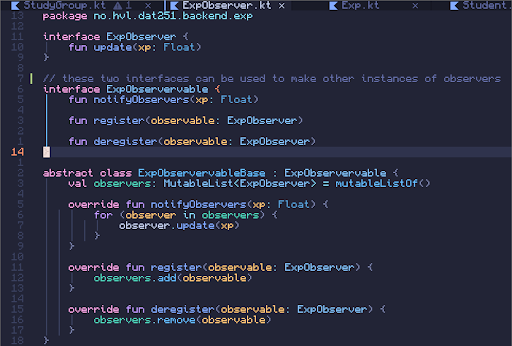
\includegraphics[width=0.7\textwidth]{images/code1}
    \caption{observer pattern}
    \label{code1}
\end{figure}
\begin{figure}[H]
    \centering
    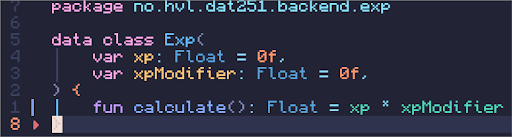
\includegraphics[width=0.7\textwidth]{images/code2}
    \caption{Exp class used in student}
    \label{code2}
\end{figure}


Since the priority was just producing code, a consequence of this was that the
parent components, such as: StudySession or StudyGroup,
would quickly become huge and tightly coupled.
As a result of this, sometimes clarity of the code was almost non-existent.


One of the refactorings in our project was splitting a
larger frontend page into smaller components with more specific responsibilities.

Before:

\begin{itemize}
\item Functionality for displaying sessions and handling session creation/editing was mainly in control of StudySession.


\end{itemize}

After:

This was split into smaller components:

\begin{itemize}
\item SessionCard for displaying a single study session

\item CreateSessionModal for handling form input and save logic.

\end{itemize}

SessionCard was created to handle the presentation of a single study session.
Including details such as subject, time, location, and actions like remove and edit.
CreateSessionModal was also created to handle the creation and editing of study sessions,
including form state, input handling, and validation logic.
This reduced the amount of responsibility that the frontend page studySession had.

This refactoring improved code quality by making the structure more modular and easier to understand.
Instead of having one large component responsible for fetching data, grouping sessions, rendering the full page,
displaying individual sessions, and handling form interaction, these responsibilities were distributed
more clearly across smaller components,
which improved readability and maintainability,
as changes to individual components have limited impact on the overall system.

This refactoring reflects the Single Responsibility Principle, since each component has a more focused role.
SessionCard is responsible for displaying a session, CreateSessionModal is responsible for session input and editing,
and studySession coordinates the state and communication with the backend.
It also reflects Separations of Concern, since presentation, form handling,
and higher-level page logic are no longer mixed together to the same extent.
This aligns with findings that refactoring can improve both code quality and developer productivity in agile teams \cite{Impact_of_Refactoring}.
This illustrates how refactoring not only improves code quality, but also helps reduce accumulated technical debt over time.